%Dokumentklasse

%draft als optionohne bilder für bessere performance
%\documentclass[a4paper,12pt,draft]{scrreprt}

%normal mit Bildern
\documentclass[a4paper,12pt]{scrreprt}

\usepackage[left= 3cm,right = 3cm, bottom = 3cm,top = 3cm]{geometry}
%\usepackage[onehalfspacing]{setspace}

% ============= Packages =============

% Dokumentinformationen
\usepackage[
	pdftitle={Praktikum - Umwelttechnik},
	pdfsubject={},
	pdfauthor={Roman-Luca Zank},
	pdfkeywords={},	
	%Links nicht einrahmen
	hidelinks
]{hyperref}

%nur Text zum prüfen des Umfangs

% Standard Packages
\usepackage[utf8]{inputenc}
\usepackage{cancel}
\usepackage[ngerman]{babel}
\usepackage[T1]{fontenc}
\usepackage{graphicx}
\graphicspath{{img/}}
\usepackage{fancyhdr}
\usepackage{lmodern}
\usepackage{color}
\usepackage{placeins}
\usepackage{booktabs}
\usepackage{caption}
\usepackage[list=true]{subcaption}
\usepackage{mhchem}

%Einheitenpackage
\usepackage{siunitx}  
\sisetup{	locale = DE, 
			per-mode=fraction,
			inter-unit-product=\ensuremath{\cdot},
			detect-weight = true,
			quotient-mode=fraction
		}
%neue Einheiten definieren
\DeclareSIUnit\xyz{xyz}	
\DeclareSIUnit\d{d}	
\DeclareSIUnit\ppm{ppm}		

%Automatisch cdot statt *
\DeclareMathSymbol{*}{\mathbin}{symbols}{"01}

%d klein in Mathemodus
\newcommand*\diff{\mathop{}\!\mathrm{d}}
\newcommand*\Diff[1]{\mathop{}\!\mathrm{d^#1}}



%\setcounter{lofdepth}{2}      %für subfigures in list of figures

%Tabelle
\usepackage{tabularx}
\usepackage{tabulary}

%%Verzeichnispackages
%\usepackage{natbib}

%\usepackage{hyperref}
%\newcites{

% zusätzliche Schriftzeichen der American Mathematical Society
\usepackage{amsfonts}
\usepackage{amsmath}

%Abkürzungsverzeichnis
\usepackage{acronym}

%kein Abstand bei neuem Kapitel vom Seitenanfang
%\vspace*{2.3\baselineskip} = ORIGINAL
\renewcommand*{\chapterheadstartvskip}{\vspace*{.0\baselineskip}}

%nicht einrücken nach Absatz
\setlength{\parindent}{0pt}

% ============= Kopf- und Fußzeile =============
\pagestyle{fancy}
%
\lhead{}
\chead{}
\rhead{}%\slshape }%\leftmark}
%%
\lfoot{}
\cfoot{}
\rfoot{\pagemark}
%%
\renewcommand{\headrulewidth}{0pt}
\renewcommand{\footrulewidth}{0pt}
\renewcommand{\chapterpagestyle}{fancy}

% ============= Package Einstellungen & Sonstiges ============= 
%Besondere Trennungen
%\hyphenation{De-zi-mal-tren-nung}
\usepackage[none]{hyphenat}
\hyphenpenalty=5000
\tolerance=5000
\providecommand\phantomsection{}

\usepackage{mathtools}

% ============= Dokumentbeginn =============

\begin{document}
%Seiten ohne Kopf- und Fußzeile sowie Seitenzahl
\pagestyle{empty}

%\begin{center}
\begin{tabular}{p{\textwidth}}


\begin{center}

\includegraphics[scale=0.75]{img/logos.jpg}\\
\end{center}


\\

\begin{center}
\LARGE{\textsc{
Protokoll \\
Umwelttechnik\\
}}
\end{center}

\\

%\begin{center}
%\large{Fakultät für Muster und Beispiele \\
%der Hochschule Musterhausen \\}
%\end{center}
%
%\\

\begin{center}
\textbf{\Large{V4 - Bodencharakterisierung}}
\end{center}

\begin{center}
	\large{Gruppe 1.2 (BCUT3)}
\end{center}


\\
%\begin{center}
%zur Erlangung des akademischen Grades\\
%Bachelor of Engineering
%\end{center}


%\begin{center}
%vorgelegt von
%\end{center}

\begin{center}
\Large{\textbf{Teilnehmer:}} \\ 
\end{center}
\begin{center}
\large{Willy Messerschmidt \\
		Roman-Luca Zank} \\
\end{center}


\\

\begin{center}
\begin{tabular}{lll}
\large{\textbf{Protokollführer:}} & & \large{Roman oder Willy} \\
& & email@stud.hs-merseburg.de\\
&&\\
\large{\textbf{Datum der Versuchsdurchführung:}}&& \large{12.12.2019}\\
&&\\
\large{\textbf{Abgabedatum:}}&& \large{12.12.2019}
\end{tabular}
\end{center}

\\ \\ \\ \\ \\ \\ \\ 
\large{Merseburg den \today}

\end{tabular}
\end{center}


%\include{14_danksagungen}

%\include{15_zusammenfassung}

% Beendet eine Seite und erzwingt auf den nachfolgenden Seiten die Ausgabe aller Gleitobjekte (z.B. Abbildungen), die bislang definiert, aber noch nicht ausgegeben wurden. Dieser Befehl fügt, falls nötig, eine leere Seite ein, sodaß die nächste Seite nach den Gleitobjekten eine ungerade Seitennummer hat. 
\cleardoubleoddpage

% Pagestyle für Titelblatt leer
\pagestyle{empty}

%Seite zählen ab
\setcounter{page}{0}

%Titelblatt
%\begin{center}
\begin{tabular}{p{\textwidth}}


\begin{center}

\includegraphics[scale=0.75]{img/logos.jpg}\\
\end{center}


\\

\begin{center}
\LARGE{\textsc{
Protokoll \\
Umwelttechnik\\
}}
\end{center}

\\

%\begin{center}
%\large{Fakultät für Muster und Beispiele \\
%der Hochschule Musterhausen \\}
%\end{center}
%
%\\

\begin{center}
\textbf{\Large{V4 - Bodencharakterisierung}}
\end{center}

\begin{center}
	\large{Gruppe 1.2 (BCUT3)}
\end{center}


\\
%\begin{center}
%zur Erlangung des akademischen Grades\\
%Bachelor of Engineering
%\end{center}


%\begin{center}
%vorgelegt von
%\end{center}

\begin{center}
\Large{\textbf{Teilnehmer:}} \\ 
\end{center}
\begin{center}
\large{Willy Messerschmidt \\
		Roman-Luca Zank} \\
\end{center}


\\

\begin{center}
\begin{tabular}{lll}
\large{\textbf{Protokollführer:}} & & \large{Roman oder Willy} \\
& & email@stud.hs-merseburg.de\\
&&\\
\large{\textbf{Datum der Versuchsdurchführung:}}&& \large{12.12.2019}\\
&&\\
\large{\textbf{Abgabedatum:}}&& \large{12.12.2019}
\end{tabular}
\end{center}

\\ \\ \\ \\ \\ \\ \\ 
\large{Merseburg den \today}

\end{tabular}
\end{center}
 %Prokolle
\begin{center}
\begin{tabular}{p{\textwidth}}


\begin{center}

\includegraphics[scale=0.75]{img/logos.jpg}\\
\end{center}


\\

\begin{center}
\LARGE{\textsc{
Organische Chemie I\\
}}
\end{center}

%\begin{center}
%\large{Fakultät für Muster und Beispiele \\
%der Hochschule Musterhausen \\}
%\end{center}
%
%\\
 \\
 
\begin{center}
\textbf{\Large{Skriptaufzeichnungen}}
\end{center}

\begin{center}
	\large{im WiSe 2019}
\end{center}
 \\
%\begin{center}
%zur Erlangung des akademischen Grades\\
%Bachelor of Engineering
%\end{center}


\begin{center}
\large{vorgelegt von}
\end{center}
\\


\begin{center}
\Large{\textbf{Roman-Luca Zank}} \\
\end{center}

\begin{center}
3. Semester \\
Chemie- und Umwelttechnik \\
\end{center}


\begin{center}
\begin{tabular}{lll}
	\textbf{E-Mail:} & & romanzank@mail.de\\
	\textbf{Matrikelnummer:} & &25240\\
	\textbf{Adresse:} & &Platz der Bausoldaten 2, Zimmer 224\\
	\textbf{Ort:} & &06217 Merseburg\\
	&& \\
	\textbf{Professor:} & & Rödel\\
\end{tabular}
\end{center}

\\ \\ \\ \\ \\
\large{Merseburg, \today}

\end{tabular}
\end{center}
 %Seminar-/Abschlussarbeit

% Pagestyle für Rest des Dokuments
\pagestyle{fancy}

%Inhaltsverzeichnis
\tableofcontents

%Inhalt

%%Verzeichnis aller Bilder
%\label{sec:bilder}
%\listoffigures
%\addcontentsline{toc}{chapter}{Abbildungsverzeichnis}

%Verzeichnis aller Tabellen
%\label{sec:tabellen}
%\listoftables
%\addcontentsline{toc}{chapter}{Tabellenverzeichnis}

%%Abkürzungsverzeichnis
%\setlength{\columnsep}{20pt}
%\twocolumn
%\addchap{Nomenklatur (fett)}
%\label{sec:abkurzung}
%\begin{acronym}
%	\acro{vbr} [\boldmath{$\dot{V}_{Br}$}] {Volumenstrom Brennstoff \\ (Erdgas)}
%	\acro{vml} [\boldmath{$\dot{V}_{L}$}] {Volumenstrom der Luft}
%	\acro{vwa} [\boldmath{$\dot{V}_{W\omega}$}] {Ausgangsvolumenstrom Wasser}
%	\\
%	\acro{mbr} [\boldmath{$\dot{m}_{Br}$}] {Massestrom Brennstoff \\ (Erdgas)}
%	\acro{ml}  [\boldmath{$\dot{m}_{L}$}] {Massenstrom Luft}
%	\acro{ma}  [\boldmath{$\dot{m}_{A}$}] {Massenstrom Abgas}
%	\acro{mwa} [\boldmath{$\dot{m}_{W\alpha}$}] {Eingangsmassenstrom Wasser}
%	\acro{mww} [\boldmath{$\dot{m}_{W\omega}$}] {Ausgangsmassenstrom Wasser}
%	\\
%	\acro{qbr} [\boldmath{$\dot{Q}_{Br}$}] {Wärmestrom Brennstoff \\ (Erdgas)}
%	\acro{qa}  [\boldmath{$\dot{Q}_{A}$}] {Wärmestrom Abgase}
%	\acro{qstr}[\boldmath{$\dot{Q}_{Str}$}] {Strahlungswärme}
%	\acro{qw}  [\boldmath{$\dot{Q}_{W}$}] {result. Wärmestrom Wasser}
%	\acro{qwe} [\boldmath{$\dot{Q}_{Weitere}$}] {Weitere Wärmeverluste}
%	\\
%	\acro{nbro} [\boldmath{$\dot{n}_{Br}$}] {Molstrom Brennstoff}
%	\acro{no2o} [\boldmath{$\dot{n}_{O_{2}}$}] {Molstrom Sauerstoff}
%	\\
%	\acro{wirkungE} [\boldmath{$\eta_{E}$}] {energetischer Wirkungsgrad}
%	\acro{wirkungF} [\boldmath{$\eta_{F}$}] {feuerungstechnischer\\ Wirkungsgrad}
%	\\
%	\acro{vT} [\boldmath{$\tau_{Vor}$}] {Heizvorlauftemperatur}
%	\acro{rT} [\boldmath{$\tau_{Rück}$}] {Heizrücklauftemperatur}
%	\acro{AT} [\boldmath{$\tau_{A}$}] {Abgastemperatur}
%	\acro{averlust} [\boldmath{$qA$}] {Abgasverlust}
%	\acro{co2}[\boldmath{$\%CO_{2}$}] {CO$_{2}$-Gehalt im Abgas}
%	\acro{o2} [\boldmath{$\%O_{2}$}] {O$_{2}$-Restgehalt im Abgas}
%	\\
%	\acro{heizbr} [\boldmath{$H_u$}$= 10,4 \frac{kWh}{m^3}$] {Heizwert \\ des Brennstoffes (Erdgas)}
%	\acro{dbr}[\boldmath{$\rho_{E}$}$= 0,7\frac{kg}{m^3}$] {Dichte \\ des Brennstoffes (Erdgas)}
%	\acro{dw} [\boldmath{$\rho_{W}$}$= 988\frac{kg}{m^3}$] {Dichte \\ des Heizfluides (Wasser)}
%	\acro{dl} [\boldmath{$\rho_{L}$}$= 1,2\frac{kg}{l}$] {Dichte der Luft}
%	\acro{cp} [\boldmath{$c_{pW}$}$= 4,1\frac{kJ}{kg*K}$] {spezifische \\ Wärmekapazität des Heizfluides (Wasser)}
%	\acro{nbr} [\boldmath{$M_{Br}= 16\frac{g}{mol}$}] {Molare Masse \\ des Brennstoffs}
%\end{acronym}
%\subsubsection{Aufrufen einer Abkürzung}
%\acs{rT}
%\begin{verbatim}
%\acs{Abkürzung}
%\end{verbatim}
%\onecolumn

\include{03_strukturbindung}

\include{04_strukturreaktion}

\include{05_alkan}
\include{06_cycloalkane}
\chapter{Stereoisomerie}

\begin{figure}[h!]
	\centering
	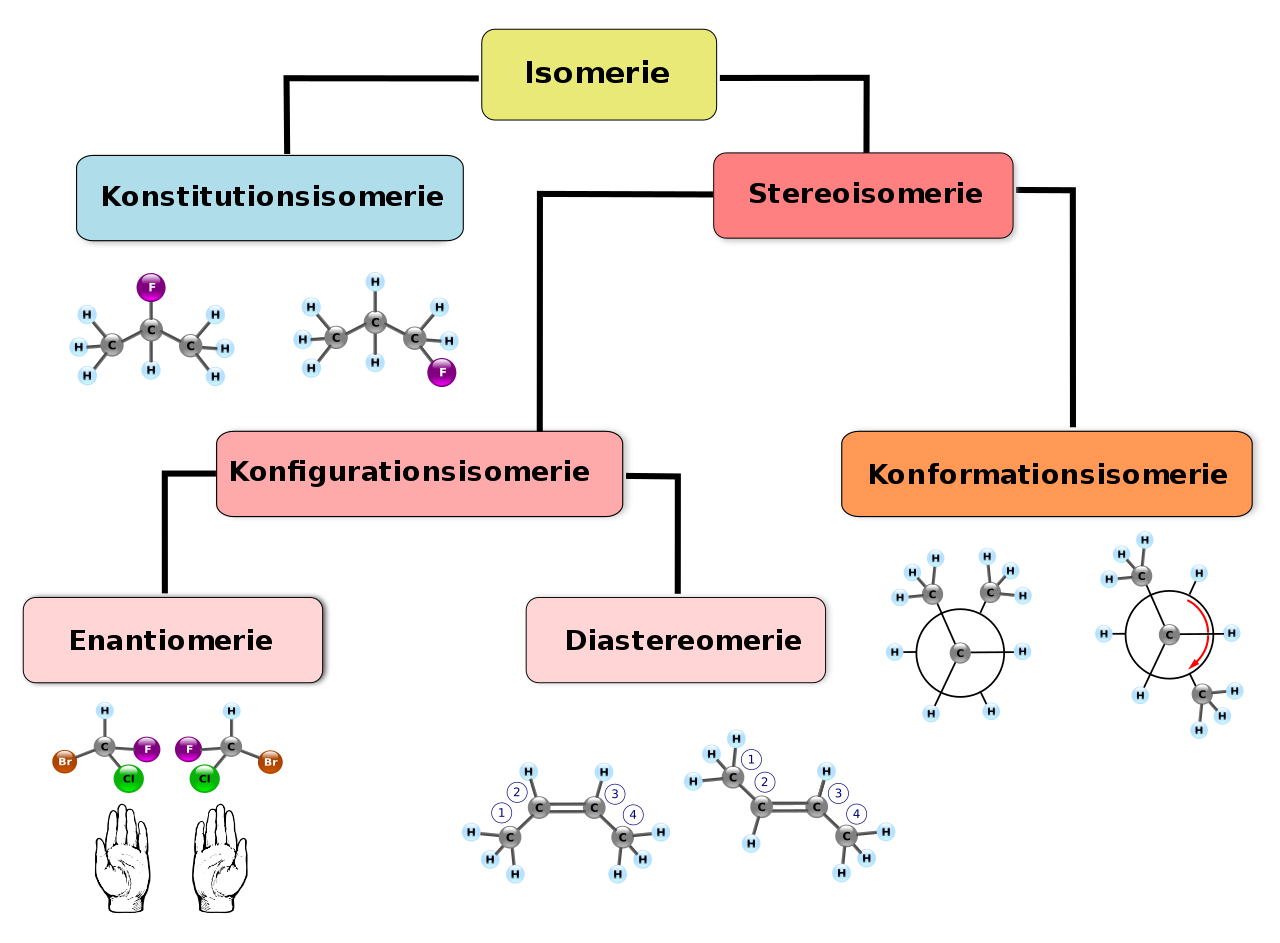
\includegraphics[width=0.75\linewidth]{img/isomerie}
	\caption{Übersicht der Isomerien}
	\label{fig:isomerie}
\end{figure}
\FloatBarrier

\begin{figure}[h!]
	\centering
	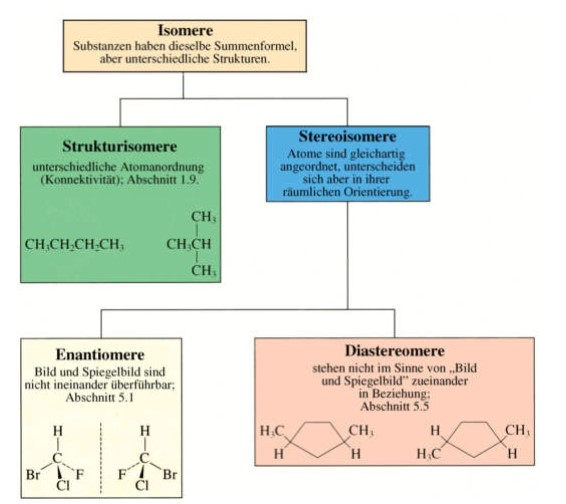
\includegraphics[width=0.75\linewidth]{img/isomerie2}
	\caption{Übersicht der Isomerien}
	\label{fig:isomerie2}
\end{figure}
\FloatBarrier

\section{Enantiomere}

\subsection{Begriffe der Enantiomere}

\textbf{{\large Chiralität:}} (griech. Händigkeit)\\
= jedes Objekt, das mit seinem Spiegelbild \textbf{nicht} zur Deckung gebracht werden kann ist chiral (nur das Molekül !)\\
$\rightarrow$ chirale Moleküle besitzen asymetrisch substituierte C-Atome als Stereozentrum
\begin{figure}[h!]
	\centering
	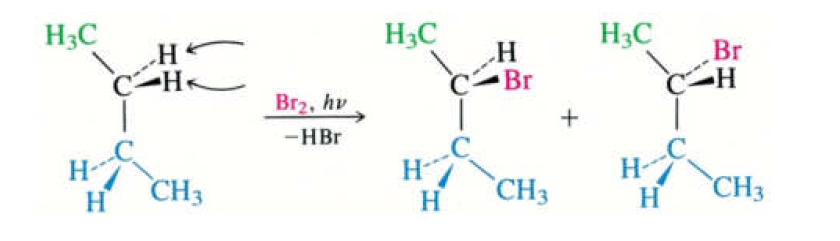
\includegraphics[width=0.75\linewidth]{img/chiral1}
	\caption{Beispielreaktion für Stereoisomere}
	\label{fig:ciral1}
\end{figure}
\FloatBarrier

\textbf{{\large Enantiomere:}} \\
= Moleküle verhalten sich wie Bild und Spiegelbild \linebreak 
 (aber nicht im Molekül selbst $\rightarrow$ sind chiral und besitzen keine molekulare Spiegelebene) \\
 $\rightarrow$ achirale Moleküle können keine Enantiomere sei, das sich Bild und Spiegelbild decken\\
 
\textbf{{\large Racemat:}} \\
= 50:50 Gemisch von Enantiomeren (L-/D-Moleküle, +/-)\\
$\rightarrow$ sind optisch inaktiv

\subsection{Unterscheidung der Enantiomere}
1. Röntgengrafische Kristallstrukturanalyse ("`Foto"')\\ 
\textbf{2. Polarimeter:} optische Rotation der Ebene des linear polarisierten Lichts


\begin{figure}[h!]
	\centering
	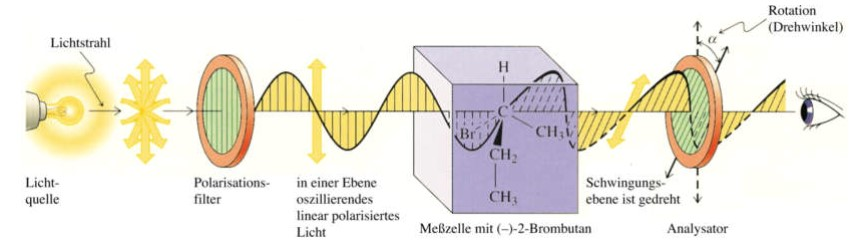
\includegraphics[width=0.75\linewidth]{img/polarimeter}
	\caption{optische Aktivität von chiralen Molekülen}
	\label{fig:polarimeter}
\end{figure}
\FloatBarrier
\begin{itemize}
	\item (+)- Enantiomer dreht sich im Uhrzeigersinn (dextrorotatorisch)
	\item (-)- Enantiomer dreht sich gegen Uhrzeigersinn (levorotatorisch)
\end{itemize}

Die Schwingungsebene des linear polarisierten Lichtes wird durch die optisch aktive Substanz am asymmetrisch substituierten C-Atom gedreht. \\
Je nachdem ob der Analysator mit oder gegen den Uhrzeigersinn dreht um das polarisierte Licht wahrzunehmen, erhält der Stoff die Bezeichnung (+/d) oder (-/l) \\

\textbf{Wichtig:} (+/d) $\neq$ D und (-/l) $\neq$ L\\

\textbf{{\large Spezifische Drehung:}}
\begin{flalign}
	\left[\alpha\right]^{\delta}_\lambda &= \frac{\alpha}{l*c}
\end{flalign}
\begin{itemize}
	\item $\left[\alpha\right]$... spezifische Drehung
	\item $\delta$... Temperatur in \si{\celsius}
	\item $\lambda$... Wellenlänge des einfallenden Lichtes
	\item $l$... Länge (in dm) der Messzelle (Küvette) 
	\item $c$... Konzentration in \si{\gram \per \milli \liter}
	\item $\alpha$... gemessene Rotation
\end{itemize}

\subsection{CIP- Sequenzregel}

\vspace*{3cm}
\textbf{{\large Fischerprojektion:}} \\

\include{08_eigenschaftenhalogenalkane}
\include{09_reaktionhalogenalkane}
\include{10_alkohole}


%\chapter*{Formelsammlung Umwelttechnik}
%
%%Emission als Massenanteil
%\begin{flalign}
%\text{\textbf{Emission (Def.)} } \text{ \textbf{:}} && \hspace*{-1em}  =\frac{\text{Schadstoff}}{\text{Produkt}} \left[\frac{\si{\kg}}{\si{t}}\right]  &&
%\end{flalign}
%
%\begin{flalign}
%\text{\textbf{Imission (Konzentration)} } \text{ \textbf{:}} && \hspace*{-1em}  =\left[\frac{\si{\kg}}{\si{\raiseto{3}\meter}}\right]  &&
%\end{flalign}
%
%\begin{flalign}
%\text{\textbf{Imission (Staubniederschlag)} } \text{ \textbf{:}} && \hspace*{-1em}  =\left[\frac{\si{\gram}}{\si{\raiseto{2}\meter*d}}\right] &&
%\end{flalign}
%
%\textbf{Ideales Gasgesetz:}
%\begin{flalign}
%& p*\dot{V}=\dot{n}*R_0*T\\
%& p*\dot{V}=\dot{m}*R_{spez.}*T\\
%& p_i*\dot{V}=\frac{\dot{m_i}}{M_i}*R_0*T
%\end{flalign}
%
%\textbf{AGW Volumenanteil $\boldsymbol{\varphi_i}$:}
%\begin{flalign}
%& = \frac{\left[\text{ppm}\right]*10^{-3}*M_i\left[\si{\gram \per \mole}\right]*1,013*10^5}{8,314*293}\left[\si{\milli \gram \per \raiseto{3} \meter}\right]\\
%&= \frac{\left[\text{ppm}\right]*M_i\left[\si{\gram \per \mole}\right]}{24,047}\left[\si{\milli \gram \per \raiseto{3} \meter}\right] \text{\small{Normbedingungen}}\\
%&= \frac{\left[\text{ppm}\right]*M_i\left[\si{\gram \per \mole}\right]}{22,4}\left[\si{\milli \gram \per \raiseto{3} \meter}\right] \text{\small{Standardbedingungen}}
%\end{flalign}
%
%\textbf{AGW Synergieeffekt:}
%\begin{flalign}
%	&= \sum_{i=1}^{n}\frac{c_i}{\text{AGW}_i} \leq 1
%\end{flalign}
%
%\textbf{AGW Arbeitstag:}
%\begin{flalign}
%& \frac{c_{\text{Zul}}}{\text{AGW}}=\frac{8h}{t_{\text{Schicht,real}}}\\
%& c_{\text{Zul}}*t_{\text{Schicht,real}}=8h*\text{{AGW}}
%\end{flalign}\\
%
%\textbf{Luftwechselzahl $\boldsymbol{l}$:}
%\begin{flalign}
%& = \frac{V_E \text{\tiny{(ausgewechselt)}}}{V_R \text{\tiny{(Raumvolumen)}}}
%\end{flalign}
%
%\textbf{Verdünnungsbelüftung (instationär) $\boldsymbol{c_i(t)}$:}
%\begin{flalign}
%&= \left(c_{i_{zu}}+\frac{\dot{m}_{i,e}}{l*V_R}\right)*\left[1-e^{-l*t}\right]+c_i(t=0)*e^{-l*t}
%\end{flalign}
%\begin{itemize}
%	\item $c_{i,max}=\frac{\dot{m}_{i,e}}{l*V_R}+c_{i,zu}$
%	\item Schadstoffkonzentration am Anfang null $c_i(t=0)=0$ 
%	\item zugeführte Luft $c_{i,zu}=0$ 
%\end{itemize}
%\textbf{Verdünnungsbelüftung (stationär) $\boldsymbol{c_i}$:}
%\begin{flalign}
%&= c_{i_{zu}}+\frac{\dot{m}_{i,e}}{l*V_R}\leq \text{AGW}_i
%\end{flalign}
%\\
%\textbf{Masse Partikel $\boldsymbol{m_p}$:}
%\begin{flalign}
%&=\rho_p*\frac{\pi}{6}*\text{x}^3
%\end{flalign}
%\\
%\textbf{Widerstand $\boldsymbol{c_W}$:}
%\begin{flalign}
%&=\frac{24}{\text{Re}}
%\end{flalign}
%\\
%\textbf{?? Stokes'sches Gesetz (Widerstandskraft) $\boldsymbol{\overrightarrow{F_W}}$:}
%\begin{flalign}
%&\overrightarrow{F_W}=\frac{3*\pi*\eta_F*\text{x}*\omega_S}{c_V}\\
%&w_S= \frac{(\varphi_P-\varphi_F)*\text{x}^2*Cu*g}{18*\eta_F}
%\end{flalign}
%\\
%\textbf{Abscheidegrad $\boldsymbol{\eta}$:}
%\begin{flalign}
%&=\frac{\dot{m}_{ab}}{\dot{m}_0}=\frac{\dot{m_0}-\dot{m}_{\tiny{Rein}}}{\dot{m_0}}\\
%\end{flalign}
%\\
%\textbf{Trenngrad $\boldsymbol{T_i(x_i)}$:}
%\begin{flalign}
%&=\frac{\dot{m}_{i,0}-\dot{m}_{i,\tiny{Rein}}}{\dot{m_{i,0}}}
%\end{flalign}
%


%Literaturverzeichnis Bücher
%\bibliography{Literatur}
%\bibliographystyle{unsrt}
%\addcontentsline{toc}{chapter}{Literaturverzeichnis}
%
%\begin{enumerate}
%	\item Praktikumsskript, Modul ………, Versuch …….., Prof. Musterprof. 
%	\item DIN 12345, Jahr der Veröffentlichung 
%	\item Link der Internetseite, Zugriffsdatum 
%	\item Buchtitel, Autor, Verlag, Veröffentlichungsjahr 
%\end{enumerate}
%
%
%
%
%
%
%%Anhang
%\addcontentsline{toc}{chapter}{Anhang}

\end{document}
